%This is part of Un soupçon de mathématique sans être agressif pour autant
% Copyright (c) 2012-2013
%   Laurent Claessens, Pauline Klein
% See the file fdl-1.3.txt for copying conditions.

Dans ce chapitre :
\begin{enumerate}
    \item
        Résoudre graphiquement des inéquations : \( f(x)\leq k\) ou \( f(x)\geq g(x)\).
    \item
        Lien tableau de variations, tableau de valeurs et dessin.
    \item
        Comparer des images depuis un tableau de variation.
    \item
        Donner des fonctions sous forme de programmes ou algos.
    \item
        Équation produit.
\end{enumerate}

%+++++++++++++++++++++++++++++++++++++++++++++++++++++++++++++++++++++++++++++++++++++++++++++++++++++++++++++++++++++++++++ 
\section{Fonction croissante et décroissante}
%+++++++++++++++++++++++++++++++++++++++++++++++++++++++++++++++++++++++++++++++++++++++++++++++++++++++++++++++++++++++++++

\begin{definition}
      Soit $f$ une fonction définie sur un intervalle \( I\) de \( \eR\).
      \begin{enumerate}
          \item 
              On dit que $f$ est \defe{croissante}{croissante (fonction)} sur $I$ si pour tout choix de réels $a$ et $b$ dans $I$ tels que $a\leq b$ nous avons $f(a)\leq f(b)$.
    \item 
        On dit que $f$ est \defe{décroissante}{décroissante (fonction)} sur $I$ si pour tout choix de $a$ et $b$ dans $I$ tels que $a\leq b$, nous avons $f(a)\geq f(b)$. 
      \end{enumerate}
\end{definition}

Une fonction croissante range les images dans le même ordre que les antécédents. Une fonction décroissante inverse cet ordre. 

\begin{example}
    Nous considérons la fonction \( f\colon x\mapsto x^2\) sur \( \eR^+\).
    \begin{equation*}
        \begin{array}[]{|c||c|}
            \hline
            x&f(x)\\
            \hline\hline
            0&0\\
            \hline
            0.1&0.01\\
            \hline
            0.5&0.25\\
            \hline
            1&1\\
            \hline
            2&4\\
            \hline
            10&100\\
            \hline
        \end{array}
    \end{equation*}
    Dans ce tableau les valeurs de \( x\) sont rangées dans l'ordre croissant et nous remarquons que les images le sont aussi. La fonction \( f(x)=x^2\) est donc croissante tant qu'on considère des nombres positifs.

    Pour les valeurs négatives c'est le contraire :
    \begin{equation*}
        \begin{array}[]{|c||c|}
            \hline
            x&f(x)\\
            \hline\hline
            -10&100\\
            \hline
            -2&4\\
            \hline
            -1&1\\
            \hline
            -0.5&0.25\\
            \hline
            -0.1&0.01\\
            \hline
            0&0\\
            \hline
        \end{array}
    \end{equation*}
    Ici les antécédents sont dans l'ordre croissant et les images sont dans l'ordre décroissant.
\end{example}
  
%+++++++++++++++++++++++++++++++++++++++++++++++++++++++++++++++++++++++++++++++++++++++++++++++++++++++++++++++++++++++++++ 
\section{Différentes manières de parler d'une fonction}
%+++++++++++++++++++++++++++++++++++++++++++++++++++++++++++++++++++++++++++++++++++++++++++++++++++++++++++++++++++++++++++

%--------------------------------------------------------------------------------------------------------------------------- 
\subsection{Tableau de valeurs}
%---------------------------------------------------------------------------------------------------------------------------

Le tableau de valeurs consiste à donner quelque valeurs connues de la fonction.

\begin{example}
    Soit une fonction \( f\) définie sur \( \mathopen[ -5 ; 10 \mathclose]\) et dont nous connaissons le tableau de valeurs suivant :
    \begin{equation}
        \begin{array}[h]{|c||c|c|c|c|c|c|}
            \hline
            x&-5&-1&1&3&9&10\\
            \hline
            f(x)&0&2&-3&7&2&5\\
            \hline
        \end{array}
    \end{equation}
    Nous pouvons dire que
    \begin{enumerate}
        \item
            L'image de \( 1\) par \( f\) est \( -3\).
        \item
            L'unique antécédent de \( 7\) est \( 3\).
        \item
            Les nombres \( -1\) et \( 9\) sont tous deux des antécédents de \( 2\).
    \end{enumerate}
    Nous ne pouvons pas dire 
    \begin{enumerate}
        \item
            L'image de \( 2\).
        \item
            Si la fonction est croissante sur \( \mathopen[ -5 ;0 \mathclose]\).
    \end{enumerate}

    En réalité n'importe quelle courbe qui passe par les points suivants peut être \( f\) :

\end{example}

WYeESAN

%--------------------------------------------------------------------------------------------------------------------------- 
\subsection{Tableau de signe}
%---------------------------------------------------------------------------------------------------------------------------

Le tableau de signe ne donne que le signe de la fonction.

%--------------------------------------------------------------------------------------------------------------------------- 
\subsection{Tableau de variations}
%---------------------------------------------------------------------------------------------------------------------------

<++>

%+++++++++++++++++++++++++++++++++++++++++++++++++++++++++++++++++++++++++++++++++++++++++++++++++++++++++++++++++++++++++++
\section{Modélisation par une fonction}
%+++++++++++++++++++++++++++++++++++++++++++++++++++++++++++++++++++++++++++++++++++++++++++++++++++++++++++++++++++++++++++

Les exemples de fonctions dans la «vraie» vie sont nombreux.

\begin{example}
    Soit un triangle rectangle isocèle dont les côtés de l'angle droit sont de longueur \( x\). Alors la surface est donnée par la fonction
    \begin{equation}
        f(x)=\frac{ x^2 }{2}.
    \end{equation}
    L'ensemble de définition est \( \defD=\mathopen] 0 , \infty \mathclose[\) parce que \( x\) représente une longueur.
\end{example}

\begin{example}
    Un vélo se déplace à \( \unit{20}{\kilo\meter\per\hour}\). Après un temps \( t\), il aura parcouru une distance
    \begin{equation}
        d(t)=20t
    \end{equation}
    kilomètres. Ici l'ensemble de définition est plus délicat; il dépend du contexte.

    Notons que la variable d'une fonction n'est pas obligatoirement toujours notée \( x\) et que la fonction n'est pas toujours obligatoirement notée \( f\).
\end{example}

\begin{example}
    Vous verrez dans un cours de physique que si on lance un objet verticalement avec une vitesse initiale \( v_0\), alors la hauteur en fonction du temps est donnée par
    \begin{equation}
        h(t)=v_0t-\frac{ gt^2 }{2}
    \end{equation}
    où \( g\) est l'accélération de la gravitation sur Terre (environ \( \unit{10}{\meter\per\second\squared}\)).
\end{example}

%---------------------------------------------------------------------------------------------------------------------------
\section{Résolution graphique d'(in)équations} 
%---------------------------------------------------------------------------------------------------------------------------

\subsection{Lecture graphique des images et des antécédents}

\begin{multicols}{2}

    Nous considérons la fonction
    \begin{equation}
        \begin{aligned}
            f\colon \eR&\to \eR \\
            x&\mapsto x^2 
        \end{aligned}
    \end{equation}
    dont le graphe est donné ci-contre. À chaque réel $x$, nous associons l'abscisse $y=f(x)$.  À l'aide du graphe donné, répondre aux questions suivantes.

    \begin{itemize}
        \item Image de $1,5$ ? 
        \item Antécédent de $3,5$ ?  
        \item Antécédent de $-1$ ? 
        \item Antécédent de $0$ ? 
    \end{itemize}

    \columnbreak

    %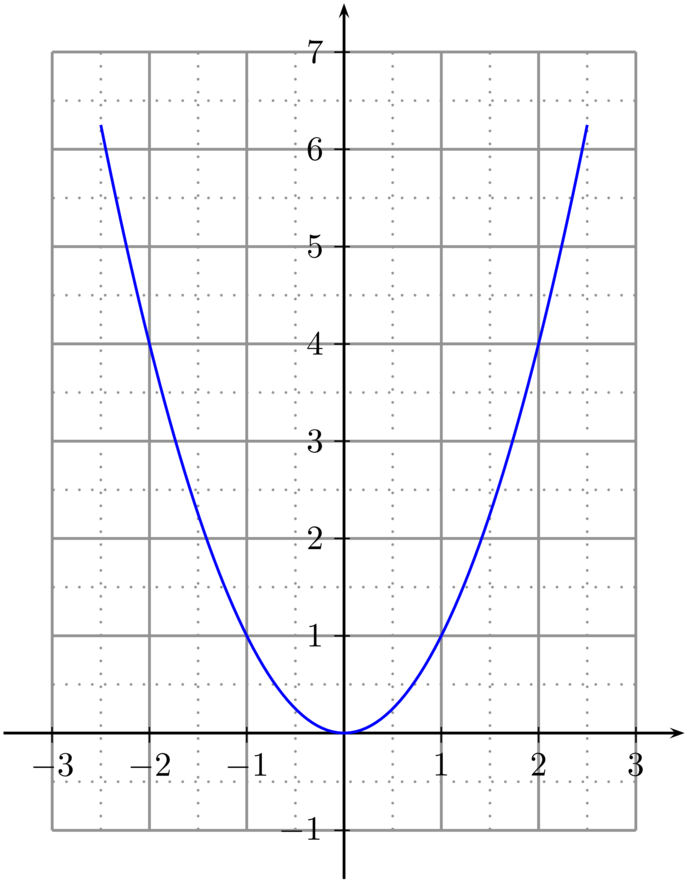
\includegraphics{Picture_FIGLabelFigFCarreQFhsWzPICTFCarreQFhsWz-for_eps.pdf}
    %\newcommand{\CaptionFigFCarreQFhsWz}{Le graphe de la fonction \( x\mapsto x^2\).}
    \input{Fig_FCarreQFhsWz.pstricks}

\end{multicols}

  \begin{example}
Compléter le tableau suivant pour la fonction $f(x)=x^2$.
\begin{equation}
\begin{array}[h]{|c|c|c|c|c|c|c|c|c|c|c|c|}
  \hline  
  x & -4 & -3 & -2 & -1 & 0 & 1 & 2 & 3 & 4 & -0,5 & 0,5  \\
  \hline
  y & 16 &&&&&&&&&&0.25\\
  \hline
\end{array}
\end{equation}
  \end{example}


\subsection{Résolution graphique d'équations}

\begin{Aretenir}
    Soit $k$, un réel fixé. Résoudre l'équation $f(x)=k$ revient à chercher les antécédents par $f$ du nombre $k$.

Le nombre de solutions de l'équation $f(x)=k$ est égal au nombre de points d'intersection de la courbe représentative de \( f\) avec la droite $d$ d'équation $y=k$. Les solutions sont les abscisses de ces points d'intersection. 
\end{Aretenir}


\begin{example}
    \begin{multicols}{2}
  Nous cherchons à résoudre $f(x)=4$. 
  \begin{itemize}
      \item 
          Nous traçons la droite horizontale d'équation \( y=4\);
      \item
          nous observons les points d'intersection de cette droite avec la courbe;
      \item
          les solutions de l'équation sont les abscisses de ces points.
  \end{itemize}

\columnbreak


%The result is on figure \ref{LabelFigExCarrexvfvre}. % From file ExCarrexvfvre
%\newcommand{\CaptionFigExCarrexvfvre}{<+Type your caption here+>}
\input{Fig_ExCarrexvfvre.pstricks}

    \end{multicols}

    Sans surprises, les solutions de \( x^2=4\) sont \( x=2\) et \( x=-2\).

\end{example}

\begin{Aretenir}
    Résoudre l'équation $f(x)=g(x)$ revient à déterminer les abscisses des points d'intersection des courbes représentatives de \( f\) et \( g\).
\end{Aretenir}


\begin{multicols}{2}

    Les solutions de l'équation \( f(x)=g(x)\) sont les abscisses des points d'intersection des deux courbes. Pour les trouver, il suffit de repérer les points d'intersections, puis de les projeter sur l'axe horizontal.

    Dans le cas de la figure ci-contre, les solutions sont approximativement \( x=-3.6\), \( x=-1.1\) et \( x=1.5\).

\columnbreak

%The result is on figure \ref{LabelFigExEquationIntersectioniSHPTw}. % From file ExEquationIntersectioniSHPTw
%\newcommand{\CaptionFigExEquationIntersectioniSHPTw}{<+Type your caption here+>}
\input{Fig_ExEquationIntersectioniSHPTw.pstricks}

\end{multicols}


\subsection{Résolution graphique d'inéquations}


%///////////////////////////////////////////////////////////////////////////////////////////////////////////////////////////
\subsubsection{Inéquation du type $f(x)<k$}
%///////////////////////////////////////////////////////////////////////////////////////////////////////////////////////////

\begin{Aretenir}
Les solutions de l'inéquation $f(x)<k$ sont les abscisses des points de $\mathscr{C}$ situés en-dessous de la droite d'équation $y=k$.

En particulier, les solutions de l'inéquation $f(x)<0$ sont les abscisses des points de la courbe représentative de \( f\) situés en-dessous de l'axe des abscisses, c'est-à-dire ayant une ordonnée strictement négative.
\end{Aretenir}

\begin{multicols}{2}
    Sur la figure ci-contre, nous résolvons \( f(x)\leq 2\). La procédure à suivre est la suivante.
    \begin{enumerate}
        \item
            Tracer la droite horizontale \( y=2\).
        \item
            Trouver les points d'intersection avec le graphe de \( f\).
        \item
            Les solutions sont les abscisses pour lesquelles le graphe de \( f\) est au-dessus du graphe de la droite \( y=2\).
    \end{enumerate}

    \columnbreak

%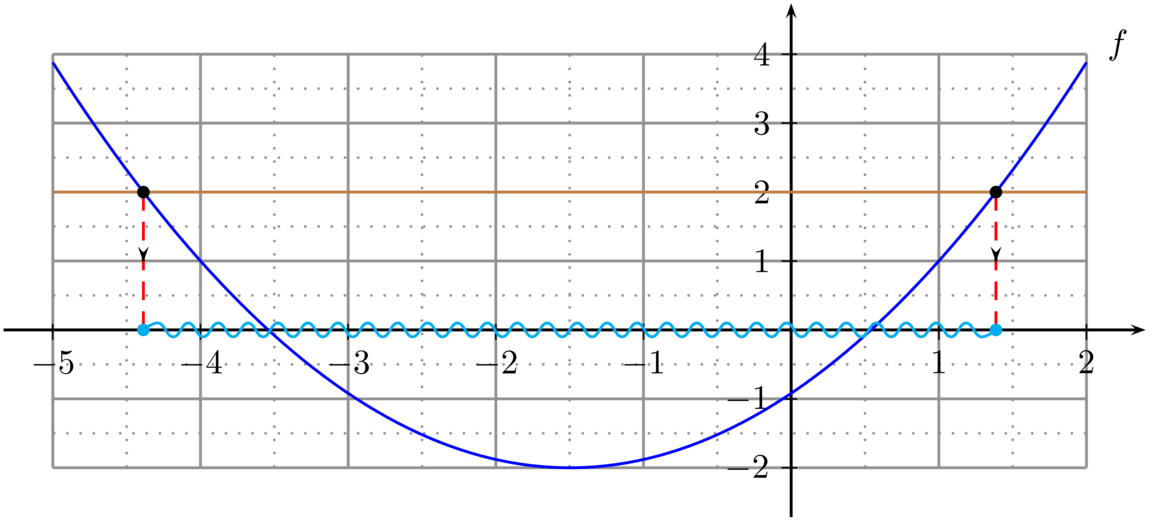
\includegraphics{Picture_FIGLabelFigExIneqOcAWMqPICTExIneqOcAWMq-for_eps.pdf}
    %\newcommand{\CaptionFigExIneqOcAWMq}{Les solutions de l'équation \( f(x)\leq 2\) sont en ondulé.}
    \input{Fig_ExIneqOcAWMq.pstricks}

\end{multicols}


\begin{remark}
    Ici nous avons résolut l'équation \( f(x)\leq 2\). Les deux points extrêmes dont partie de l'ensemble des solutions. Si nous avions résolu \( f(x)<2\), alors les points extrêmes n'auraient pas fait partie de l'ensemble des solutions.
\end{remark}

On procède de la même manière pour les inégalités du type $f(x)>k$, $f(x)\geq k$, $f(x)\leq k$. 

%///////////////////////////////////////////////////////////////////////////////////////////////////////////////////////////
\subsubsection{Inéquation du type $f(x)<g(x)$}
%///////////////////////////////////////////////////////////////////////////////////////////////////////////////////////////

Les solutions de l'inéquation $f(x)<g(x)$ sont les abscisses des points pour lesquels la courbe de \( f\) est en-dessous de la courbe de \( g\).

\newcommand{\CaptionFigExIneqfgZWStde}{En cyan, l'ensemble des solutions de l'inéquation \( f(x)<g(x)\).}
\input{Fig_ExIneqfgZWStde.pstricks}

La figure \ref{LabelFigExIneqfgZWStde} montre la résolution d'une telle inéquation. Notons que l'ensemble des solutions peut être en plusieurs morceaux.


\subsection{Tableau de variations}


Le \defe{tableau de variation}{tableau de variation} est un tableau contenant
\begin{enumerate}
    \item
        les positions des sommets,
    \item
        les flèches indiquant les endroits où la fonction est croissante ou décroissante.
\end{enumerate}
Un petit exemple valant mieux qu'un long discours\ldots

% à noter le 9 dans l'environnement suivant est le nombre de lignes sur lesquelles la figure s'étale. Je suis obligé de donner à la main parce que le tableau ne compte apparemment que pour une seule ligne. Du coup si je laisse à LaTeX le soin de calculer, les lignes de texte en-dessous de la figure (et en particulier à la page suivante si la figure est en bas de page) sont encore coupées.
\begin{wrapfigure}[9]{r}{6.0cm}     
   \vspace{-1cm}        % à adapter.
   \centering
   \input{Fig_GrapheVarREGMqx.pstricks}
\end{wrapfigure}

    Le tableau de variation de la fonction dessinée ci-contre est :
    \begin{equation*}
    \begin{array}[h]{|c|ccccccc|}
        \hline
        x&-3&&-2&&0&&2\\
        \hline
        &&&2&&&&1\\
        f(x)&&\nearrow&&\searrow&&\nearrow&\\
        &-\frac{ 9 }{2}&&&&-\frac{ 1 }{2}&&\\
        \hline
    \end{array}
    \end{equation*}
    En effet, la fonction \( f\)
    \begin{itemize}
        \item 
            part de \( x=-3\) où \( f(x)=-9/2\);
        \item
            elle monte jusqu'en \( x=-2\) où elle vaut \( f(x)=2\);
        \item
            elle descend jusqu'en \( x=0\) où elle vaut \( -\frac{ 1 }{2}\);
        \item
            elle monte jusqu'en \( x=2\) où elle vaut \( 1\).
    \end{itemize}

Le plus souvent si on donne un dessin, les nombres à placer dans un tableau de variation sont des valeur approchées à la précision du dessin. Donner les réponses en fraction n'est donc pas obligatoire. Par exemple ici au lieu d'écrire \( -9/2\) dans le tableau, il aurait été possible d'écrire \( -4.5\).

\section{Minimum et maximum}

Les notions de minima et maxima parlent, comme l'indiquent leurs noms en français, des points du graphe d'une fonction les plus hauts et les plus bas.

\begin{definition}
      Soit $f$ une fonction définie sur un intervalle $I$.
      \begin{itemize}
          \item On dit que $f$ admet le réel $m$ pour \defe{minimum}{minimum (d'une fonction)} sur $I$ si et seulement si il existe $c\in I$ tel que $f(c)=m$ et pour tout $x\in I$, $f(x)\geq m$. 
    \item On dit que $f$ admet le réel $M$ pour \defe{maximum}{maximum} sur $I$ si et seulement si il existe $d\in I$ tel que $f(d)=M$ et pour tout $x\in I$, $f(x)\leq M$.
      \end{itemize}
\end{definition}

%Sur la figure \ref{LabelFigMinMaxKNRdOd}, nous avons indiqué le minimum et le maximum de la fonction dessinée.
%\newcommand{\CaptionFigMinMaxKNRdOd}{Minimum et maximum d'une fonction.}
Sur le dessin ci-dessous nous avons indiqué le minimum et le maximum de la fonction dessinée.
\input{Fig_MinMaxKNRdOd.pstricks}

%+++++++++++++++++++++++++++++++++++++++++++++++++++++++++++++++++++++++++++++++++++++++++++++++++++++++++++++++++++++++++++ 
\section{Pour tracer}
%+++++++++++++++++++++++++++++++++++++++++++++++++++++++++++++++++++++++++++++++++++++++++++++++++++++++++++++++++++++++++++

Quelque conseils pour dessiner.
\begin{itemize}
    \item
        Pour une valeur $x$ sur l'axe des abscisses, il y a un et un seul point d'abscisse $x$ sur la courbe.
    \item
        Pour tracer une courbe, il faut placer des points. Plus on choisit de points, plus la courbe sera précise.
    \item
        Si possible, trouver quelque valeurs clefs. Par exemple on cherchera les points d'intersection entre les axes et les courbe. Le point \( (0,f(0)) \) est intéressant à mettre, ainsi que les points \( x\) tels que \( f(x)=0\).
\end{itemize}


\newcommand{\CaptionFigExFonction}{Comment tracer la fonction \( f\colon x\to 2x+1\) ?}
\input{Fig_ExFonction.pstricks}

Nous donnons à la figure \ref{LabelFigExFonction} le tracé de la fonction \( f(x)=2x+1\). La figure \ref{LabelFigExFonctionssLabelSubFigExFonction0} donne quelque points du graphe de la fonction. La figure \ref{LabelFigExFonctionssLabelSubFigExFonction1} donne le graphe complet de la fonction. Comment le construit-on ? Par définition pour chaque \( x\) sur l'axe des abscisses (il y en a une infinité), il faut calculer le nombre \( f(x)\) et mettre dans le plan le point de coordonnées \( \big( x,f(x) \big)\).

En pratique, il n'est pas possible de calculer \( f(x)\) pour \emph{tous} les \( x\) réels\footnote{Chuck Norris peut le faire.}. C'est pourquoi nous nous contentons qu'en calculer quelque uns, et nous les relions «le plus intelligemment possible».


%---------------------------------------------------------------------------------------------------------------------------
\subsection{Ce qui n'est pas une fonction}
%---------------------------------------------------------------------------------------------------------------------------

%    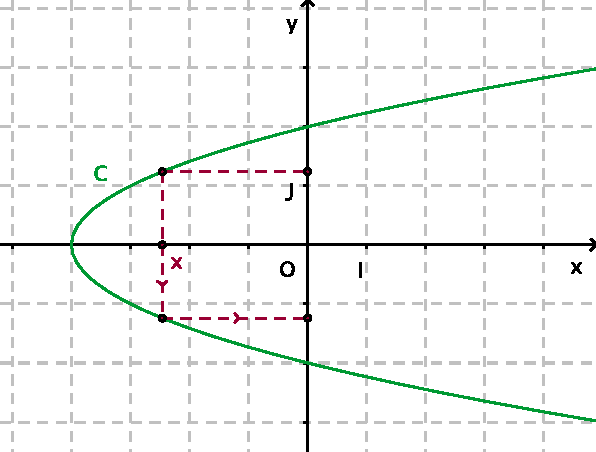
\includegraphics[width=5cm]{F_NonFct.pdf}

\begin{multicols}{2}
    Cette courbe ne représente pas une fonction, car à partir de \( x=-4\), les nombres ont deux images. Les courbes données par des fonctions sont des courbes acceptant une seule ordonnée pour chaque abscisse.

\columnbreak

%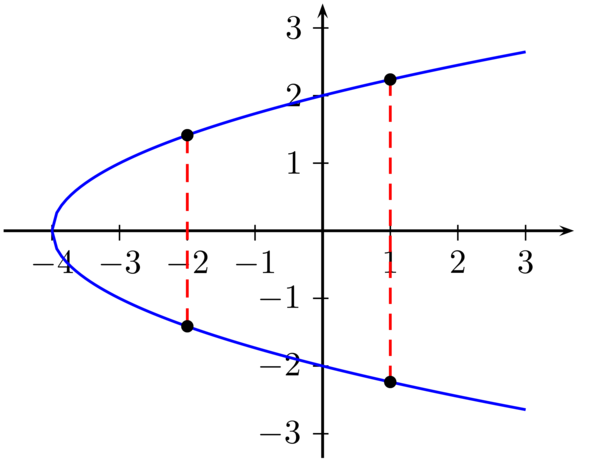
\includegraphics{Picture_FIGLabelFigPasFonctionYoQfSuPICTPasFonctionYoQfSu-for_eps.pdf}

\input{Fig_PasFonctionYoQfSu.pstricks}

\end{multicols}


Pour tracer le graphe d'une fonction affine.
\begin{itemize}
    \item
        Vu que le graphe est une droite, il suffit de deux points.
    \item
        Les fonction linéaires passent par l'origine \( (0;0)\).
    \item 
        Pour un tracé à la règle, il est plus précis de prendre deux points relativement éloignés.
    \item
        La droite \( f(x)=mx+p\) monte si \( m>0\) et descend si \( m<0\). La pente est d'autant plus forte que \( m\) est grand.
\end{itemize}

Quelque exemples à la figure \ref{LabelFigGrapheAffinHqXJGx}.
\newcommand{\CaptionFigGrapheAffinHqXJGx}{Des graphes de fonctions linéaires et affines.}
\input{Fig_GrapheAffinHqXJGx.pstricks}
